\section{El programa Agenda telefónica}

\begin{itemize}
  \item El programa necesita guardar los datos que el usuario dispone, estos datos deben ser almacenados en algún tipo de archivos. Debido a que se necesitan guardar listas de objetos, se ha decidido hacer uso de archivos JSON, un formato ligero de intercambio de datos, fácil de leer y escribir con la biblioteca json de Python, adecuado para datos estructurado.
  \item Leer y escribir en archivos con Python viene de forma nativa y se utiliza a través de las funciones integradas \mpy{open}, \mpy{read}, \mpy{write} entre otras. Sin embargo para manejar ciertos formatos especificos como JSON, Python ofrece el modulo estándar json.
\end{itemize}

\subsection{La clase Contacto}
Contiene los campos mencionados necesarios para identificar al contacto

\begin{minted}[bgcolor=background]{python}
def __init__(self, nombre: str, telefono: str, direccion: str, relacion: str):
  self._nombre = nombre
  self._telefono = telefono
  self._direccion = direccion
  self._relacion = relacion
\end{minted}

Además debe de contener los métodos que se llaman automaticamente al momento de representar como string al objeto actual.

\begin{minted}[bgcolor=background]{python}
def __repr__(self) -> str:
  return self.__str__()

def __str__(self) -> str:
  return (f"\nNombre:\t\t{self._nombre}\nTelefono:\t{self._telefono}\n"
          f"Direccion:\t{self._direccion}\nRelacion:\t{self._relacion}\n")
\end{minted}

Debemos de tener un método que nos permita parsear el objeto actual como un diccionario. Por ejemplo, que el identificador de referencia al campo name sea como clave y su valor sea el correspondiente valor del campo.

\begin{minted}[bgcolor=background]{python}
def parsear_a_json(self):
  return {
    "nombre": self.nombre,
    "telefono": self.telefono,
    "direccion": self.direccion,
    "relacion": self.relacion
  }
\end{minted}

Un método que reciba como argumento un diccionario, basicamente es el objeto JSON parseado por el modulo json de Python. Este diccionario contiene los campos de una instancia de la clase Contact, por lo tanto con estos datos se debe crear el nuevo objeto. Si analizamos, este método será parte de cargar los datos guardados en un archivo JSON.

\begin{minted}[bgcolor=background]{python}
@staticmethod
def parsear_de_json(dic):
  return Contacto(dic["nombre"], dic["telefono"], dic["direccion"], dic["relacion"])
\end{minted}

El método debe de ser estático porque necesitamos acceder a este mismo sin tener que crear aún un objeto Contacto.

\subsection{La clase Agenda}
Esta clase contiene un campo \mpy{self._contacts} que es una lista de objetos Contacto. Aqui tenemos una particularidad a destacar. Se decidió que el \textbf{archivo que guarda los contactos se recupera automáticamente} al momento de crear una instancia de esta clase.

\begin{minted}[bgcolor=background]{python}
def __init__(self, path_data):
  self._contacts = self.recuperar_agenda(path_data)
\end{minted}

Por lo tanto, comenzaremos explicando el método \mpy{recuperar_agenda()}.

\subsubsection{El método \mpy{recuperar_agenda(path_data)}}
La lógica es recuperar el archivo con la dirección que nosotros como desarrolladores han decidido, en caso no exista el archivo, entonces se regresa una lista vacíá; de lo contrario necesitamos cargar el archivo.

\begin{minted}[bgcolor=background]{python}
def recuperar_agenda(self, path_data):
  if not (os.path.exists(path_data)):
    return []

  with open(path_data, "r") as data: 
    datos = json.load(data)
    print("Recuperación exitosa...\n")
  return [Contacto.parsear_de_json(dic) for dic in datos]
\end{minted}

Cuando cargamos el archivo, este se carga en diccionarios, ya que la conversión de objetos JSON es a diccionarios en Python. Entonces aqui debemos de utilizar el método \mpy{parsear_de_json()} que recibe el diccionario y crear con estos valores el objeto Contacto. 

\subsubsection{El método \mpy{getContact(pattern)}}
Básicamente la lógica consiste en iterar sobre las lista \mpy{self._contacts} y recuperar su campo \mpy{nombre}.
\singlespacing
Ahora necesitamos comparar dicho nombre con el patrón ingresado. Para resolver este problema se ha utilizado el siguiente algoritmo.

\paragraph{Algoritmo de Knuth-Morris-Pratt (KMP):}
El algoritmo KMP utiliza la información del propio patrón para evitar retrocesos innecesarios en la cadena de texto. Esto se logra mediante la construcción de un arreglo de prefijo (función de prefijo o función $\pi$), también conocido como "arreglo de fallos" o "tabla de fallos", que se utiliza para saltar comparaciones redundantes.

\begin{figure}[H]
  \centering
  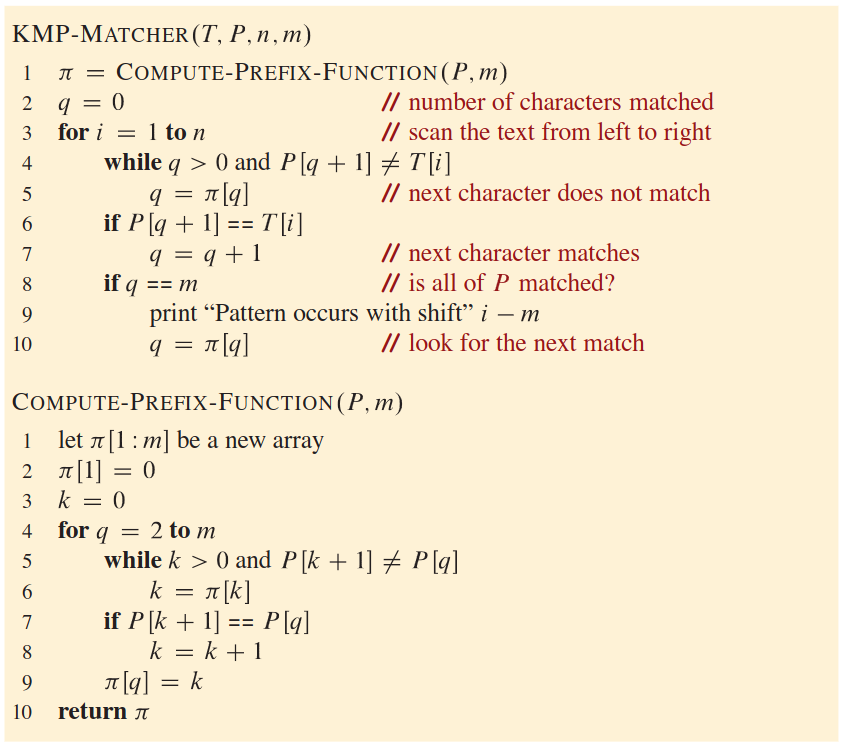
\includegraphics[width=0.8\textwidth]{img/kmp.png}
  \caption{Pseudocodigo del algoritmo KMP}
\end{figure}

Entonces en ves de devolver el indice de la primera posición de la cadena de texto de todas las coincidencias, nosotros hemos hecho que devuelva \mpy{True} o \mpy{False}.


\begin{minted}[bgcolor=background]{python}
# Algoritmo Knuth-Morris-Pratt (KMP)
def _match(self, name, pattern):
  lps = self._compute_lps(pattern)
  i = 0
  j = 0

  while i < len(name):
    if pattern[j] == name[i]:
      i += 1
      j += 1

    if j == len(pattern):
      j = lps[j - 1]
      return True
    elif i < len(name) and pattern[j] != name[i]:
      if j != 0:
        j = lps[j - 1]
      else:
        i += 1
  return False

# Generación de la funcion $\pi$
def _compute_lps(self, pattern):
  lps = [0] * len(pattern)
  length = 0
  i = 1

  while i < len(pattern):
    if pattern[i] == pattern[length]:
      length += 1
      lps[i] = length
      i += 1
    else:
      if length != 0:
        length = lps[length - 1]
      else:
        lps[i] = 0
        i += 1
  return lps
\end{minted}

\subsubsection{El método \mpy{guardar_agenda()}}
El método consiste en iterar en los objetos de la lists \mpy{self._contacts} y generar una lista ya no de objetos Contacto, sino ahora una lista de diccionarios, usando el método \mpy{parsear_a_json()} de la clase Contacto.

\begin{minted}[bgcolor=background]{python}
def guardar_agenda(self):
  contacts_pars = [contact.parsear_a_json() for contact in self._contacts]
  with open("./data/data.json", "w", encoding = "utf-8") as save:
    json.dump(contacts_pars, save, ensure_ascii=False, indent=2)
    print("Guardacion exitosa...\n")
\end{minted}
